% COMPILER: pdfLaTeX
\documentclass[12pt,a4paper,twoside,openright]{book}

\usepackage[a4paper,twoside,width=150mm,top=35mm,bottom=35mm,bindingoffset=6mm]{geometry}
\usepackage[utf8]{inputenc}
\usepackage[T1]{fontenc}
\usepackage[italian]{babel}
\usepackage{caption}
\usepackage{parskip}
\usepackage[printonlyused]{acronym}
\usepackage[hidelinks]{hyperref}
\usepackage{emptypage}
\usepackage{amsmath}
\usepackage{graphicx}
\usepackage[svgnames]{xcolor}
\usepackage[nocheck]{fancyhdr}
\usepackage{fancyvrb}
\usepackage[Lenny]{fncychap}
\usepackage{minted}


\hypersetup{
    pdftitle={Integrazione di funzionalità su infrastruttura virtuale SLURM},
    pdfsubject={Tirocinio T, Amministrazione di Sistemi T},
    pdfauthor={Massimo Valerio Zerbini - 0000969932},
    pdfkeywords={SLURM, Cluster, Vagrant, Ansible, Networking}
}

\pagestyle{fancy}
% Default document-wide minted style:
\setminted{style=default,frame=lines,framesep=2mm,rulecolor=darkgray,baselinestretch=1.2,bgcolor=WhiteSmoke,fontsize=\footnotesize,linenos,breaklines,highlightcolor=LemonChiffon}
% Language-specific minted styles:
\setminted[properties]{style=sas}
\setminted[console]{linenos=false,frame=leftline}
\setminted[yaml]{escapeinside=||}


\begin{document} % ================================================================
\begin{titlepage}
\begin{center}
    \textbf{
        {ALMA MATER STUDIORUM -- UNIVERSITÀ DI BOLOGNA\\}
        \vspace{4mm}
        SCUOLA DI INGEGNERIA E ARCHITETTURA\\ (SEDE DI BOLOGNA)\\
        \vspace{4mm}
        Anno Accademico 2024/2025
        \vspace{5mm}
        \rule{\linewidth}{0.4mm}
        {\large RELAZIONE DI FINE TIROCINIO CURRICULARE}\\
    }
    \vspace{10mm}
    {\small \textbf{svolto dallo studente:}}\\
    \vspace{2mm}
    \textsc{\textsl{Massimo Valerio Zerbini (matricola: 0000969932)}}\\
    \vspace{4mm}
    {\small \textbf{iscritto al Corso di Studio in:}}\\
    \vspace{2mm}
    \textsc{\textsl{Ingegneria Informatica T (codice: 9254)}}\\
    \vspace{4mm}
    {\small \textbf{presso:}}\\
    \vspace{2mm}
    \textsc{\textsl{ULISSE --- Dipartimento di Informatica -- Scienza e Ingegneria (DISI)}}\\
    \vspace{4mm}
    {\small \textbf{sul seguente argomento:}}\\
    \vspace{2mm}
    \textsc{\textsl{Integrazione di funzionalità su infrastruttura virtuale SLURM}}\\
\end{center}
\vfill
\begin{minipage}[t]{0.47\textwidth}
    {\small \textbf{Studente:}}\\
    \rule[-0.8cm]{0.9\linewidth}{0.1mm}\\
    {\scriptsize (firma)}
\end{minipage}
\hfill
\begin{minipage}[t]{0.47\textwidth}
    \vspace{3cm}
    \raggedleft{
        {\small \textbf{Tutor Accademico \& \\Referente Struttura Ospitante:}\\
        \vspace{1mm}
        \textsc{\textsl{Prof. Marco Prandini}}}\\
        \rule[-0.8cm]{0.9\linewidth}{0.1mm}\\
        {\scriptsize (firma per approvazione della relazione finale)}\\
    }
\end{minipage}
\vfill
\end{titlepage}

\tableofcontents

\chapter{\textbf{Introduzione}} % =================================================
\section{Obiettivi}
L'attività di tirocinio svolta presso il gruppo \ac{ULISSE} del \ac{DISI} ha avuto come obiettivo lo sviluppo di un ambiente virtuale distribuito per l'integrazione di funzionalità relative al settore del \ac{HPC}. In particolare, si è richiesta l'implementazione di:
\begin{itemize}
    \item \textbf{federazione di \textit{cluster}}, ossia il coordinamento tra molteplici infrastrutture per l'esecuzione di calcoli;
    \item \textbf{condivisione delle risorse di computazione} disponibili, al fine di raggiungere il pieno utilizzo della potenza di calcolo dei nodi;
    \item \textbf{priorità di \textit{scheduling}} per un determinato utente, ristretta a una risorsa di computazione specifica.
\end{itemize}

\section{Tecnologie coinvolte}
Le competenze richieste per la realizzazione del progetto sono basate principalmente sul corso di Amministrazione di Sistemi. L'attività di studio e documentazione sui nuovi strumenti è stata autonomamente svolta online. Di seguito vengono presentate le principali tecnologie utilizzate.

\subsection{Git}
Git è un \ac{VCS} distribuito, in grado di registrare i cambiamenti durante lo sviluppo di un progetto, mantenendone la cronologia. È caratterizzato da una gestione efficiente e scalabile delle informazioni. Il principale vantaggio nell'uso dei \ac{VCS} è dato dal forte supporto allo sviluppo non lineare, che permette la diramazione (``\textit{branching}'') e la successiva fusione (``\textit{merging}'') di nuove funzionalità.

Git si basa sul concetto di \textit{repository}, ovvero una ``copia'' del progetto. Per la collaborazione tra sviluppatori viene spesso utilizzato un repository remoto, sempre accessibile; il singolo sviluppatore lavora (anche offline) sulla propria copia locale e, quando lo ritiene opportuno, aggiorna il repository remoto. GitHub e GitLab sono esempi di servizi che offrono hosting di repository remoti.

\subsection{Vagrant}
Vagrant è un software di gestione di \ac{VM} focalizzato sulla riproducibilità affidabile degli ambienti virtualizzati. Dipende da programmi di virtualizzazione esterni (detti ``\textit{provider}''), come VirtualBox e VMware, ma risulta portabile rispetto a essi.

L'immagine di una \ac{VM} di base (denominata ``\textit{box}'') è facilmente reperibile da un deposito online contenente un'ampia varietà di sistemi operativi. Vagrant fa utilizzo di un file di configurazione (\texttt{Vagrantfile}) per ottenere i parametri di esecuzione.

\subsection{Ansible}
Ansible è un software di configurazione automatica di ambienti informatici, nota come \ac{IaC}. Ansible lavora in architettura ``\textit{agentless}'', dove il controllore comunica ed esegue le operazioni necessarie (``\textit{provisioning}'') su uno o più nodi oggetto, mediante una semplice connessione \ac{SSH} e senza quindi l'esigenza di software specifico sui nodi da configurare (escludendo il server \ac{SSH}).

Ansible utilizza i ``\textit{playbook}'', un elenco di istruzioni da eseguire che coinvolgono i nodi destinatari. I playbook sono scritti in linguaggio \ac{YAML}, di facile interpretazione.

\subsection{MariaDB}
MariaDB è un \ac{DBMS} relazionale, utilizzato per l'interfacciamento con un \ac{DB}. MariaDB è basato su MySQL, estendendone le funzionalità e migliorandone le prestazioni.

\subsection{MUNGE}
\ac{MUNGE} è un servizio di autenticazione per la creazione e validazione di credenziali utente, progettato appositamente per l'uso in ambienti \ac{HPC}. La codifica e decodifica delle credenziali si basa su una chiave comune, condivisa ai soli nodi fidati.

\subsection{SLURM}
\ac{SLURM} è un software di gestione e coordinamento di nodi di calcolo, finalizzato alla pianificazione e l'esecuzione di programmi (``\textit{jobs}''). \ac{SLURM} è altamente scalabile, rendendolo adatto anche in contesti \ac{HPC} a elevato uso di risorse. Di default utilizza \ac{MUNGE} per l'autenticazione dei nodi.

\ac{SLURM} integra tre funzioni principali:
\begin{itemize}
    \item allocazione esclusiva (e non) delle risorse computazionali agli utenti, per un periodo di tempo configurabile;
    \item inclusione di un \textit{framework} per la sottomissione e il monitoraggio dell'esecuzione di programmi;
    \item gestione della contesa di risorse mediante una coda di esecuzione.
\end{itemize}
È possibile includere funzionalità aggiuntive, quali registrazione delle attività (``\textit{accounting}'') e limitazione dell'uso di risorse, tramite il caricamento di \textit{plugin} opzionali.

\subsubsection{Architettura}
Un cluster \ac{SLURM} è coordinato dal demone controllore \texttt{slurmctld}, il cui compito è gestire le richieste di esecuzione e le risorse disponibili. Ciascun nodo di calcolo esegue \texttt{slurmd} per comunicare con il controllore ed effettuare i task richiesti. Il demone \texttt{slurmdbd}, connesso a un \ac{DBMS}, diventa essenziale per la registrazione in un singolo \ac{DB} delle attività di molteplici cluster.
\begin{figure}[ht]
    \centering
    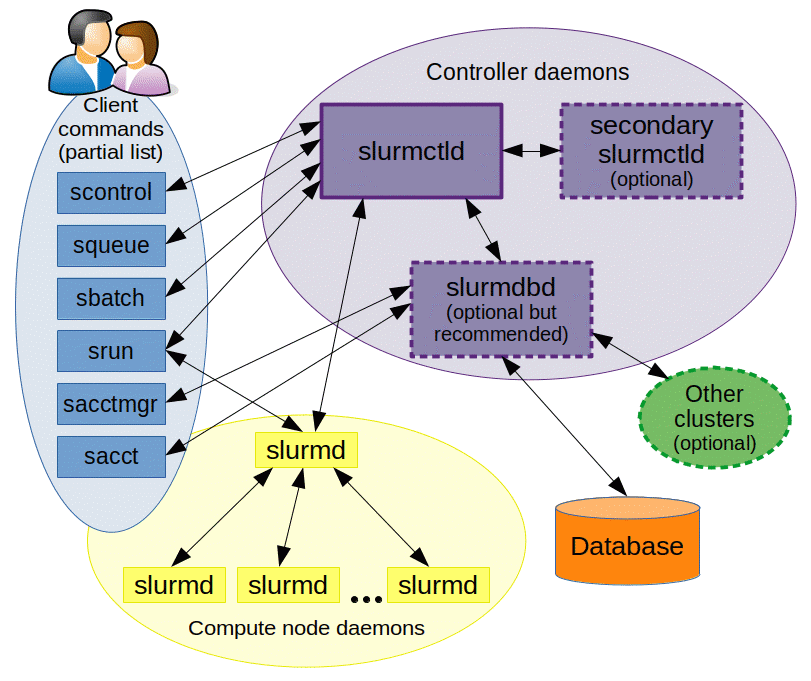
\includegraphics[width=0.7\linewidth]{images/slurm_architecture.png}
    \caption{Componenti \ac{SLURM}}
    \label{fig:slurm-components}
\end{figure}

\subsubsection{Federazione}
\ac{SLURM} permette la creazione di federazioni di cluster, dove la sottomissione dei job viene inoltrata a tutti i componenti. Ciascun cluster tenta dunque di portare a termine la richiesta di esecuzione, in modo indipendente. Per il corretto coordinamento all'interno della federazione è necessario che tutte le istanze di \texttt{slurmctld} (una per cluster) possano comunicare tra loro, oltre che con la singola istanza di \texttt{slurmdbd}, dedicata alla registrazione delle attività.
\begin{figure}[ht]
    \centering
    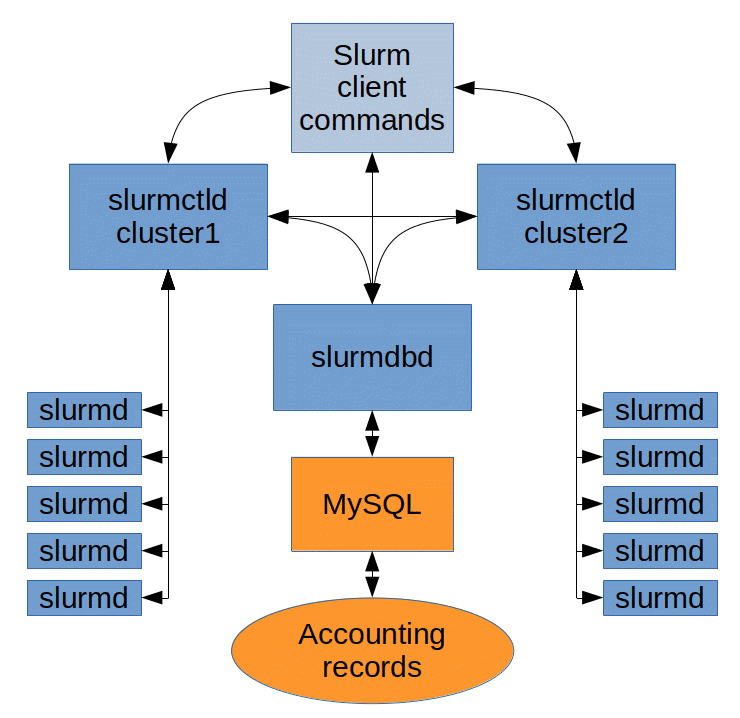
\includegraphics[width=0.55\linewidth]{images/network_federation.png}
    \caption{Comunicazione in una federazione \ac{SLURM}}
    \label{fig:slurm-federation-network}
\end{figure}


\chapter{\textbf{Attività svolte}} % ==============================================
\section{Repository}
Per lo sviluppo del progetto mi è stato concesso l'accesso a un repository Git remoto sulla piattaforma GitLab interna al \ac{DISI}, autenticandomi da pagina web con le credenziali istituzionali.

Affinché potessi lavorare su copia locale e salvare le modifiche sul repository remoto, è stato necessario generare una chiave asimmetrica \ac{SSH} e inserire la parte pubblica nel mio account GitLab. In seguito, ho aggiunto una voce \textit{host} al file locale di configurazione \ac{SSH}, per indicare a \texttt{git} come autenticarsi correttamente:
\begin{minted}[label=/home/max/.ssh/config]{properties}
...
Host gitlab.disi.unibo.it
  User git
  PreferredAuthentications publickey
  IdentityFile /home/max/.ssh/id_gitlab_unibo
...
\end{minted}
Ho quindi istanziato una copia locale del progetto (``\textit{cloning}''). Il repository conteneva una prima stesura di un cluster virtuale \ac{SLURM}, con un nodo controllore e due nodi worker. Come da prassi nello sviluppo software di nuove funzionalità, ho anzitutto generato un nuovo \textit{branch}, denominato ``tirocinio'', sul quale avrei lavorato da quel momento in poi.

\section{Risoluzione DNS}
Prima di estendere l'infrastruttura con un secondo cluster, ho dovuto verificare il funzionamento di quello già presente. \ac{SLURM} basa le proprie comunicazioni sugli \textit{hostname} e non su indirizzi \ac{IP}: ciò implica una corretta risoluzione \ac{DNS}, ovvero la ``traduzione'' da nome a indirizzo \ac{IP} corrispondente.

Come \ac{DNS} \textit{resolver} ho scelto \texttt{dnsmasq}, un software leggero in grado di svolgere anche la funzione di \ac{DHCP} server, per l'assegnamento automatico degli indirizzi \ac{IP} in una \ac{LAN}. Il programma viene eseguito su \texttt{controller}, con indirizzo \ac{IP} statico \texttt{192.168.10.254}, e su cui è presente il file di configurazione:
\begin{minted}[label=dnsmasq.conf]{properties}
interface=eth1
no-hosts
no-resolv

# NAMESERVER USED FOR THE INTERNET (host running the VMs)
server=10.0.2.3

dhcp-range=192.168.10.1,192.168.10.253,12h
dhcp-option-force=option:dns-server,192.168.10.254
\end{minted}
In questo modo i nodi worker (denominati \texttt{slurm1} e \texttt{slurm2}) ottengono un indirizzo \ac{IP} all'interno del range, causando la registrazione della corrispondenza \textit{hostname}:\textit{indirizzo}. Nel momento in cui si richiede la risoluzione di un nome di host, \texttt{dnsmasq} risponde con l'indirizzo \ac{IP} associato.

\section{MariaDB \& \texttt{slurmdbd}}
Essendo prevista la registrazione delle attività (\textit{accounting}) in contesti multi-cluster \ac{SLURM}, è stata necessaria la configurazione di un \ac{DB} e relativo \ac{DBMS} (in questo caso, MariaDB).

Per non esporre credenziali nei file utilizzati da Ansible, sono state definite delle apposite variabili di esecuzione:
\begin{minted}[label=secrets.yml]{yaml}
mariadb:
  root_password: THIS_IS_THE_ROOT_DB_PASSWORD
  slurm_password: THIS_IS_THE_SLURM_DB_PASSWORD
\end{minted}
Al fine di semplificare e isolare l'installazione del \ac{DB} su \texttt{controller}, è stato utilizzato il software di containerizzazione \texttt{podman}, che recupera ed esegue l'immagine di MariaDB opportunamente configurata:
\begin{minted}[label=roles/mariadb/tasks/main.yml]{yaml}
|\textcolor{black}{...}|
- name: Pull a MariaDB container
  become: true
  become_user: 'mariadb'
  containers.podman.podman_image:
    name: 'mariadb:latest'

- name: Run MariaDB container
  become: true
  become_user: 'mariadb'
  containers.podman.podman_container:
    name: 'mariadb'
    image: 'mariadb:latest'
    state: started
    ports: "127.0.0.1:3306:3306"
    env:
        MARIADB_ROOT_PASSWORD: "{{ mariadb.root_password }}"
|\textcolor{black}{...}|
\end{minted}
In questo modo MariaDB risulta in ascolto sulla porta \ac{TCP} \texttt{3306} di \texttt{controller}.

Seguendo poi la documentazione \ac{SLURM} per il corretto interfacciamento tra il \ac{DBMS} e \texttt{slurmdbd}, si generano \ac{DB} e utente dedicati:
\begin{minted}[label=roles/mariadb/tasks/main.yml]{yaml}
|\textcolor{black}{...}|
- name: Ensure 'slurm_db' database is present
  community.mysql.mysql_db:
    name: slurm_db
    state: present
    login_host: 127.0.0.1
    login_port: 3306
    login_user: root
    login_password: "{{ mariadb.root_password }}"
  retries: 6
  delay: 10

# NOTE: wildcard '%' (any host) as host for 'slurm' is necessary to connect via
# TCP/IP ports
- name: Ensure 'slurm' MySQL user is present with password
  community.mysql.mysql_user:
    name: slurm
    password: "{{ mariadb.slurm_password }}"
    host: '%'
    login_host: 127.0.0.1
    login_user: root
    login_password: "{{ mariadb.root_password }}"
    state: present
|\textcolor{black}{...}|
\end{minted}
Si impostano poi i privilegi appropriati, assicurandosi che vengano salvati e applicati (``\textit{flushing}''):
\begin{minted}[label=roles/mariadb/tasks/main.yml]{yaml}
|\textcolor{black}{...}|
- name: Grant usage privilege to the user
  community.mysql.mysql_user:
    name: slurm
    priv: '*.*:USAGE'
    append_privs: yes
    host: '%'
    login_host: 127.0.0.1
    login_user: root
    login_password: "{{ mariadb.root_password }}"
    state: present

- name: Grant all privileges on the database to the user
  community.mysql.mysql_user:
    name: slurm
    priv: 'slurm_db.*:ALL'
    append_privs: yes
    host: '%'
    login_host: 127.0.0.1
    login_user: root
    login_password: "{{ mariadb.root_password }}"
    state: present

- name: Flush privileges (update & reload grant tables)
  community.mysql.mysql_user:
    login_user: root
    login_password: "{{ mariadb.root_password }}"
    check_implicit_admin: yes
    append_privs: yes
    login_host: 127.0.0.1
    state: present
    name: slurm
    host: '%'
|\textcolor{black}{...}|
\end{minted}
A questo punto ho verificato manualmente l'accesso al \ac{DB} presentandomi come user \texttt{slurm}, lo stesso che verrà poi utilizzato da \texttt{slurmdbd}:
\begin{minted}{console}
vagrant@controller:~$ mariadb -u slurm --port=3306 --password=THIS_IS_THE_SLURM_DB_PASSWORD slurm_db
Reading table information for completion of table and column names
You can turn off this feature to get a quicker startup with -A

Welcome to the MariaDB monitor.  Commands end with ; or \g.
Your MariaDB connection id is 12
Server version: 11.5.2-MariaDB-ubu2404 mariadb.org binary distribution

Copyright (c) 2000, 2018, Oracle, MariaDB Corporation Ab and others.

Type 'help;' or '\h' for help. Type '\c' to clear the current input statement.

MariaDB [slurm_db]>_
\end{minted}
Ho quindi proseguito installando il demone stesso e importando il file di configurazione specifico:
\begin{minted}[label=roles/mariadb/tasks/main.yml]{yaml}
|\textcolor{black}{...}|
- name: Install 'slurmdb' package
  ansible.builtin.apt:
    name: 'slurmdbd'
    update_cache: true

- name: Copy slurmdb config file 
  ansible.builtin.template:
    src: 'slurmdbd.conf'
    dest: '/etc/slurm/slurmdbd.conf'
    mode: '0600'
    owner: 'slurm'
    group: 'slurm'
\end{minted}
Il file di configurazione per \texttt{slurmdbd} era così composto:
\begin{minted}[label=slurmdbd.conf]{properties}
AuthType=auth/munge
DbdHost=controller
DbdPort=6819
DebugLevel=verbose
StorageHost=localhost
StorageLoc=slurm_db
StoragePass="{{ mariadb.slurm_password }}"
StoragePort=3306
StorageType=accounting_storage/mysql
StorageUser=slurm
LogFile=/var/log/slurm/slurmdbd.log
PidFile=/run/slurmdbd.pid
SlurmUser=slurm
\end{minted}
Nel tentativo di avviare il demone si sono però presentati i seguenti messaggi di errore:
\begin{minted}[highlightlines=4]{console}
vagrant@controller:~$ sudo slurmdbd -D -vvv
slurmdbd: debug2: accounting_storage/as_mysql: init: mysql_connect() called for db slurm_db
slurmdbd: debug2: Attempting to connect to localhost:3306
slurmdbd: error: mysql_real_connect failed: 2002 Can't connect to local server through socket '/run/mysqld/mysqld.sock' (2)
slurmdbd: error: The database must be up when starting the MYSQL plugin.  Trying again in 5 seconds.
\end{minted}
Indagando sull'errore evidenziato ho appreso che \texttt{slurmdbd}, nel momento in cui si specifica \mintinline{properties}{StorageHost=localhost}, tenta la connessione al \ac{DB} tramite \textit{socket} locale di default (\texttt{/run/mysqld/mysqld.sock}). Eseguendo però il \ac{DBMS} all'interno di un container, la posizione della socket diventa relativa al \textit{filesystem} ``virtuale'':
\begin{minted}[breakanywhere]{console}
vagrant@controller:~$ sudo find / -type s | grep 'mysqld.sock'
/home/mariadb/.local/share/containers/storage/overlay/e7d63d4ddde910afaf1d2574c3345fc74c42372bffc95f84528ead29c2f52d7e/diff/run/mysqld/mysqld.sock
\end{minted}
Ho così aggiornato il file di configurazione:
\begin{minted}[label=slurmdbd.conf]{properties}
...
StorageHost=127.0.0.1
...
\end{minted}
In questo modo il demone viene forzato a utilizzare porte \ac{TCP}/\ac{IP} per stabilire la connessione al \ac{DB}. Ora \texttt{slurmdbd} viene avviato senza errori.

\section{Cluster singolo}
Nel seguente file di configurazione, utilizzato da entrambi \texttt{slurmctld} e \texttt{slurmd}, viene descritto il generico comportamento del cluster:
\begin{minted}[label=slurm.conf]{properties}
ClusterName=cluster
SlurmctldHost=controller
MpiDefault=none
ProctrackType=proctrack/cgroup
ReturnToService=1
SlurmctldPidFile=/var/run/slurmctld.pid
SlurmctldPort=6817
SlurmdPidFile=/var/run/slurmd.pid
SlurmdPort=6818
SlurmdSpoolDir=/var/slurm/slurmd
SlurmUser=slurm
SlurmdUser=root
StateSaveLocation=/var/slurm/slurmctld
SwitchType=switch/none
TaskPlugin=task/affinity
#
# SCHEDULING
SchedulerType=sched/backfill
SelectType=select/linear
#
# LOGGING AND ACCOUNTING
AccountingStorageType=accounting_storage/slurmdbd
JobAcctGatherType=jobacct_gather/none
SlurmctldLogFile=/var/log/slurm/slurmctld.log
SlurmdLogFile=/var/log/slurm/slurmd.log
#
# COMPUTE NODES
NodeName=slurm[1-2] CPUs=4 State=UNKNOWN
PartitionName=debug Nodes=ALL Default=YES MaxTime=INFINITE State=UP
\end{minted}
Avendo indicato \mintinline{properties}{AccountingStorageType=accounting_storage/slurmdbd}, \texttt{slurmctld} attiva la registrazione delle attività comunicando con \texttt{slurmdbd}, tramite la porta di default \texttt{6819}.

Per verificare l'intero funzionamento del cluster è necessario anzitutto avviare i nodi worker (\texttt{slurm1} e \texttt{slurm2}), che si collegano in automatico al controllore, risolvendo il nome di host indicato da \mintinline{properties}{SlurmctldHost=controller}. In particolare, la comunicazione avviene sulla porta di default \texttt{6817}. Una volta attivi, si può verificare lo stato dei nodi eseguendo:
\begin{minted}{console}
vagrant@controller:~$ sinfo
PARTITION AVAIL  TIMELIMIT  NODES  STATE NODELIST
debug*       up   infinite      2   idle slurm[1-2]
\end{minted}
Un esempio di sottomissione di job è il seguente (l'opzione \texttt{-N} indica il numero di nodi worker su cui svolgere il comando):
\begin{minted}{console}
vagrant@controller:~$ srun -N2 hostname
slurm1
slurm2
\end{minted}
È quindi evidente che il programma \texttt{hostname} sia stato eseguito da entrambi i nodi di computazione, confermando il corretto funzionamento del cluster.

\section{Topologia di rete}
Una federazione \ac{SLURM}, per definizione, è composta da (almeno) due cluster in comunicazione tra loro; in contesti reali, è verosimile che ciascuno di essi venga confinato all'interno della propria \ac{LAN}, dove la trasmissione verso l'esterno è mediata da un \textit{router}. Il seguente schema visualizza il concetto, applicandolo al caso di tirocinio:
\begin{figure}[ht]
    \centering
    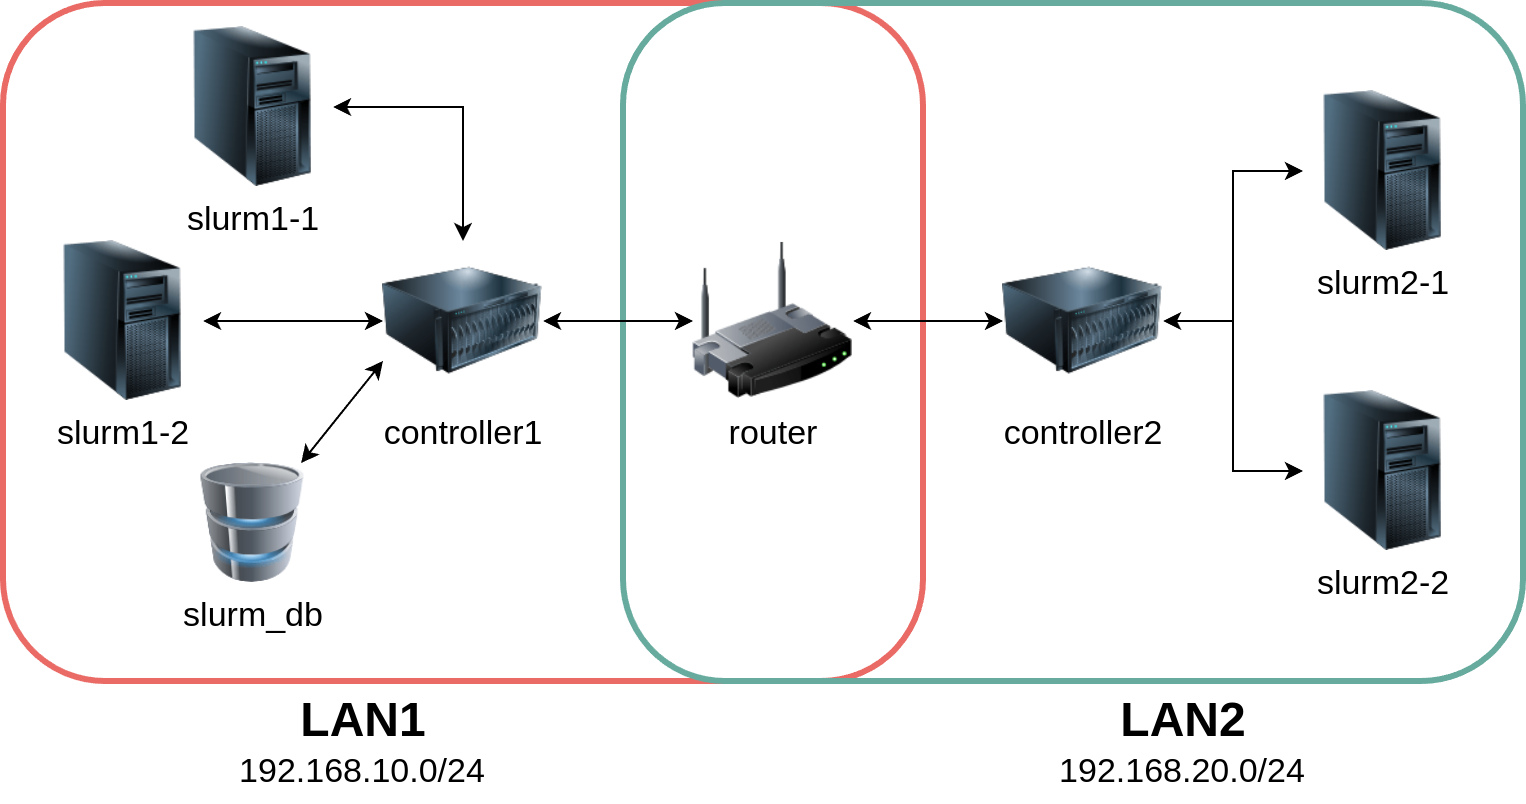
\includegraphics[width=0.9\linewidth]{images/topology.png}
    \caption{Topologia virtuale desiderata}
    \label{fig:topology}
\end{figure}

Ho dunque esteso l'infrastruttura con una seconda rete di host virtuali e un'ulteriore \ac{VM} per svolgere la funzione di router. Il file di configurazione di Vagrant risulta così composto:
\begin{minted}[label=Vagrantfile]{ruby}
Vagrant.configure("2") do |config|
  #
  # VM BOX CONFIGURATION
  config.vm.box = "debian/bookworm64"
  config.vm.provider "virtualbox" do |vb|
    vb.linked_clone = true
    vb.memory = "2048"
    vb.cpus = "4"
  end
  #
  # VIRTUAL MACHINES
  config.vm.define "router" do |machine|
    machine.vm.hostname = "router"
    machine.vm.network "private_network", virtualbox__intnet: "LAN1", auto_config: false
    machine.vm.network "private_network", virtualbox__intnet: "LAN2", auto_config: false
  end
  (1..2).each do |i|
    config.vm.define "controller#{i}" do |machine|
      machine.vm.hostname = "controller#{i}"
      machine.vm.network "private_network", virtualbox__intnet: "LAN#{i}", auto_config: false
    end
    (1..2).each do |j|
      config.vm.define "slurm#{i}-#{j}" do |machine|
        machine.vm.hostname = "slurm#{i}-#{j}"
        machine.vm.network "private_network", virtualbox__intnet: "LAN#{i}", auto_config: false
      end
    end
  end
  #
  # PROVISIONING
  config.vm.provision "ansible" do |ansible|
    ansible.playbook = "site.yml"
  end
end
\end{minted}
Da notare l'uso di iterazioni per la definizione compatta di molteplici \ac{VM}.

Ho assegnato a \texttt{router} gli indirizzi \ac{IP} statici \texttt{192.168.10.254} e \texttt{192.168.20.254}, su due interfacce separate; essendo appartenente a entrambe le \ac{LAN}, ho poi trasferito su di esso l'esecuzione di \texttt{dnsmasq}, modificandone la configurazione per servire richieste \ac{DHCP} e \ac{DNS} originanti da entrambe le reti:
\begin{minted}[label=dnsmasq.conf,highlightlines=19]{properties}
interface=eth1
interface=eth2
no-hosts
no-resolv

# NAMESERVER USED FOR THE INTERNET (host running the VMs)
server=10.0.2.3

dhcp-range=interface:eth1,192.168.10.1,192.168.10.253,12h
dhcp-range=interface:eth2,192.168.20.1,192.168.20.253,12h

dhcp-option-force=interface:eth1,option:dns-server,192.168.10.254
dhcp-option-force=interface:eth2,option:dns-server,192.168.20.254

# AVOID ROUTING ALL TRAFFIC THROUGH THIS VM
dhcp-option=3

# STATIC ROUTE FOR CROSS-LAN COMMUNICATION
dhcp-option=121,192.168.20.0/24,192.168.10.254,192.168.10.0/24,192.168.20.254
\end{minted}
L'opzione evidenziata specifica il \textit{gateway} tra le reti, ossia il ``percorso'' da scegliere in caso di pacchetti provenienti da una \ac{LAN} e destinati all'altra. Affinché \texttt{router} possa effettivamente instradare i pacchetti, è necessario attivare il \textit{forwarding} a livello di kernel:
\begin{minted}[label=roles/router/tasks/main.yml]{yaml}
|\textcolor{black}{...}|
- name: Allow IPv4 forwarding
  ansible.builtin.lineinfile:
    path: '/etc/sysctl.conf'
    line: 'net.ipv4.ip_forward=1'
    state: present
  notify: Reload kernel config
|\textcolor{black}{...}|
\end{minted}
Ora l'infrastruttura è pronta per l'integrazione del secondo cluster \ac{SLURM}.

\section{Federazione SLURM}
Ciascun cluster \ac{SLURM} è descritto interamente dal file \texttt{slurm.conf} corrispondente, che deve risultare identico su tutti i nodi. Dovendo separare l'ambiente, ho generato due file di configurazione indipendenti; di seguito sono indicate le loro differenze rispetto alla struttura a cluster singolo:
\begin{minted}[label=roles/cluster1/templates/slurm.conf]{properties}
# CLUSTER 1 CONFIG
ClusterName=cluster1
SlurmctldHost=controller1
FederationParameters=fed_display
...
NodeName=slurm1-[1-2] ...
...
\end{minted}
\begin{minted}[label=roles/cluster2/templates/slurm.conf,highlightlines=6]{properties}
# CLUSTER 2 CONFIG
ClusterName=cluster2
SlurmctldHost=controller2
FederationParameters=fed_display
...
AccountingStorageHost=controller1
...
NodeName=slurm2-[1-2] ...
...
\end{minted}
L'opzione evidenziata, presente solo nel cluster senza \ac{DB}, indica l'host dove viene eseguito \texttt{slurmdbd}, da contattare per l'\textit{accounting} delle attività. La registrazione di entrambi i cluster sullo stesso \ac{DB} è una prerogativa essenziale per l'impostazione della federazione:
\begin{minted}{console}
vagrant@controller1:~$ sudo sacctmgr add federation testfederation clusters=cluster1,cluster2
 Adding Federation(s)
  testfederation
 Settings
  Cluster       = cluster1
  Cluster       = cluster2
Would you like to commit changes? (You have 30 seconds to decide)
 (N/y): y
\end{minted}
Utilizzando \texttt{sacctmgr} e \texttt{scontrol}, ho confermato la corretta comunicazione tra i due cluster:
\begin{minted}{console}
vagrant@controller1:~$ sacctmgr show federation
Federation    Cluster ID             Features     FedState
---------- ---------- -- -------------------- ------------
testfeder+   cluster1  1                            ACTIVE
testfeder+   cluster2  2                            ACTIVE
vagrant@controller1:~$ scontrol show federation
Federation: testfederation
Self:       cluster1:127.0.0.1:6817 ID:1 FedState:ACTIVE Features:
Sibling:    cluster2:192.168.20.194:6817 ID:2 FedState:ACTIVE Features: PersistConnSend/Recv:Yes/Yes Synced:Yes
\end{minted}
Il comando \texttt{sinfo} presenta ora anche lo specifico cluster di provenienza dei nodi:
\begin{minted}{console}
vagrant@controller1:~$ sinfo
PARTITION CLUSTER  AVAIL  TIMELIMIT  NODES  STATE NODELIST
debug*    cluster1    up   infinite      1   idle slurm1-[1-2]
debug*    cluster2    up   infinite      1   idle slurm2-[1-2]
\end{minted}
Grazie all'opzione \texttt{{-}{-}clusters} in fase di sottomissione, è possibile specificare una lista di cluster sulla quale tentare di eseguire il job richiesto:
\begin{minted}{console}
vagrant@controller1:~$ srun --clusters=cluster2 -N2 hostname
slurm2-1
slurm2-2
vagrant@controller2:~$ srun --clusters=cluster1 -N2 hostname
slurm1-1
slurm1-2
\end{minted}
Da notare come, in entrambe le sottomissioni di esempio, il controllore di partenza non appartenga al cluster specificato per l'esecuzione, verificando quindi il corretto comportamento della federazione.

\section{Condivisione di risorse}
La seconda funzionalità richiesta dal tirocinio riguarda la condivisione delle risorse di computazione dei nodi, in particolare di \ac{CPU}, \ac{RAM} e \ac{GPU}. La configurazione del comportamento è descritta in \texttt{slurm.conf} e può raggiungere alti livelli di personalizzazione, in base alle esigenze specifiche.

Allo scopo di semplificare l'implementazione, ho lavorato su un singolo cluster \ac{SLURM}, composto da nodo controllore e nodo di computazione. La configurazione presenta le aggiunte:
\begin{minted}[label=slurm.conf]{properties}
...
SelectType=select/cons_tres
SelectTypeParameters=CR_CPU_Memory
...
AccountingStorageTRES=gres/gpu
...
GresTypes=gpu
NodeName=worker CPUs=4 RealMemory=1024 Gres=gpu:rtx2080ti:2 State=UNKNOWN
...
\end{minted}
In particolare, le seguenti opzioni specificano:
\begin{itemize}
    \item \mintinline{properties}{SelectType=select/cons_tres}: plugin apposito per la gestione delle risorse (``\textit{consumable trackable resources}'') e quindi l'esecuzione di più job sullo stesso nodo;
    \item \mintinline{properties}{SelectTypeParameters=CR_CPU_Memory}: risorse da condividere (la \ac{GPU} viene contata separatamente);
    \item \mintinline{properties}{AccountingStorageTRES=gres/gpu}: registrazione dell'attività delle \ac{GPU};
    \item \mintinline{properties}{GresTypes=gpu}: tipi di \ac{GRES} da condividere;
    \item \mintinline{properties}{RealMemory=1024}: memoria totale (in \ac{MB}) allocabile per nodo worker (opzione obbligatoria per la condivisione della memoria; deve essere minore o uguale alla \ac{RAM} riconosciuta dal sistema operativo);
    \item \mintinline{properties}{Gres=gpu:rtx2080ti:2}: specifiche \ac{GRES} presenti nel nodo (in questo caso, due \ac{GPU}).
\end{itemize}
È stato poi necessario introdurre nel nodo \texttt{worker} due ulteriori file di configurazione, per l'interfacciamento con le risorse presenti:
\begin{minted}[label=cgroup.conf]{properties}
CgroupPlugin=autodetect
CgroupAutomount=yes
ConstrainCores=no
ConstrainRAMSpace=no
ConstrainDevices=yes
\end{minted}
\begin{minted}[label=gres.conf]{properties}
NodeName=worker Name=gpu Type=rtx2080ti Count=2 File=/dev/nvidia[0-1]
\end{minted}
A questo punto, tramite il comando \texttt{sinfo}, ho controllato la presenza delle giuste risorse nel nodo di computazione:
\begin{minted}{console}
vagrant@controller:~$ sinfo -o "%15N  %10c  %10m  %20G"
NODELIST         CPUS        MEMORY      GRES
worker           4           1024        gpu:rtx2080ti:2
\end{minted}
Per verificare il funzionamento, ho allocato quattro job da 1 \ac{CPU} (\texttt{-c1}) e 256 \ac{MB} di \ac{RAM} (\texttt{{-}{-}mem=256}):
\begin{minted}{console}
vagrant@controller:~$ srun -c1 --mem=256 sleep 60 &
[1] 18254
vagrant@controller:~$ srun -c1 --mem=256 sleep 60 &
[2] 18264
vagrant@controller:~$ srun -c1 --mem=256 sleep 60 &
[3] 18274
vagrant@controller:~$ srun -c1 --mem=256 sleep 60 &
[4] 18284
\end{minted}
Con il comando \texttt{squeue} ho poi accertato l'esecuzione contemporanea dei job (tutti in stato \textit{running}) sul nodo \texttt{worker} da 4 \ac{CPU} e 1 GB di \ac{RAM}, a dimostrazione della condivisione dei processori e della memoria:
\begin{minted}{console}
vagrant@controller:~$ squeue
JOBID PARTITION     NAME     USER ST       TIME  NODES NODELIST(REASON)
    1     debug    sleep  vagrant  R       0:15      1 worker
    2     debug    sleep  vagrant  R       0:14      1 worker
    3     debug    sleep  vagrant  R       0:13      1 worker
    4     debug    sleep  vagrant  R       0:12      1 worker
\end{minted}
Allo stesso modo, ho allocato due job richiedenti 1 \ac{GPU} ciascuno (\texttt{{-}{-}gpus=1}) e verificato la loro esecuzione parallela:
\begin{minted}{console}
vagrant@controller:~$ srun --gpus=1 --mem=256 sleep 60 &
[1] 18294
vagrant@controller:~$ srun --gpus=1 --mem=256 sleep 60 &
[2] 18304
vagrant@controller:~$ squeue
JOBID PARTITION     NAME     USER ST       TIME  NODES NODELIST(REASON)
    5     debug    sleep  vagrant  R       0:08      1 worker
    6     debug    sleep  vagrant  R       0:07      1 worker
\end{minted}

\section{Priorità di scheduling}
La terza funzionalità richiesta dal tirocinio è stata l'impostazione della priorità di esecuzione per uno specifico utente, su una singola \ac{GPU} del nodo di computazione. L'idea di base consiste nel generare un'ulteriore partizione \ac{SLURM}, prioritaria (tramite \ac{QOS}), attiva su una \ac{GPU} e accessibile solo dall'utente desiderato.

Sono partito definendo degli utenti/gruppi di test, coerenti su ciascun nodo del cluster; nel mio caso ho scelto \texttt{user1} come utente prioritario:
\begin{minted}[label=roles/slurmcommon/tasks/main.yml]{yaml}
|\textcolor{black}{...}|
- name: Ensure test groups exist
  ansible.builtin.group:
    name: "{{ item.name }}"
    gid: "{{ item.id }}"
    state: present
  loop:
    - { name: 'user1', id: '2001' }
    - { name: 'user2', id: '2002' }
    - { name: 'user3', id: '2003' }
    - { name: 'user4', id: '2004' }

- name: Ensure test users exist
  ansible.builtin.user:
    name: "{{ item.name }}"
    uid: "{{ item.id }}"
    group: "{{ item.name }}"
    state: present
  loop:
    - { name: 'user1', id: '2001' }
    - { name: 'user2', id: '2002' }
    - { name: 'user3', id: '2003' }
    - { name: 'user4', id: '2004' }
|\textcolor{black}{...}|
\end{minted}
Il file di configurazione \ac{SLURM} è stato modificato in questo modo:
\begin{minted}[label=slurm.conf]{properties}
...
PriorityType=priority/multifactor
PriorityWeightQOS=10000
PriorityWeightTRES=GRES/gpu=100
...
AccountingStorageEnforce=limits
JobAcctGatherType=jobacct_gather/cgroup
...
PartitionName=gpupart Nodes=worker QOS=gpuprio AllowAccounts=user1acct State=UP
\end{minted}
In particolare, le seguenti opzioni specificano:
\begin{itemize}
    \item \mintinline{properties}{PriorityType=priority/multifactor}: plugin che coinvolge più fattori per determinare la priorità di un job; per il caso in questione ho aumentato il peso di \ac{QOS} e \ac{GPU}, tramite le opzioni \texttt{PriorityWeight-};
    \item \mintinline{properties}{AccountingStorageEnforce=limits}: imposizione dei limiti (sulle risorse) descritti nel \ac{DB}; impone inoltre, per tutte le richieste di esecuzione di job, la presenza di un'associazione (utente, account, partizione, ...) valida;
    \item \mintinline{properties}{PartitionName=gpupart}: partizione aggiuntiva ristretta all'account \texttt{user1acct}, con \ac{QOS} \texttt{gpuprio}.
\end{itemize}
Ho dunque registrato nel \ac{DB} (tramite il comando \texttt{sacctmgr}) le informazioni per il comportamento desiderato:
\begin{minted}{console}
vagrant@controller:~$ sudo sacctmgr add qos gpuprio Priority=10 GrpTRES=gres/gpu=1
 Adding QOS(s)
  gpuprio
 Settings
  Description    = gpuprio
  GrpTRES                  = gres/gpu=1
  Priority                 = 10
Would you like to commit changes? (You have 30 seconds to decide)
 (N/y): y
vagrant@controller:~$ sudo sacctmgr add account user1acct QOS=gpuprio
 Adding Account(s)
  user1acct
 Settings
  Description     = Account Name
  Organization    = Parent/Account Name
 Associations =
  C = testcluster A = user1acct
 Settings
  QOS           = gpuprio
Would you like to commit changes? (You have 30 seconds to decide)
 (N/y): y
vagrant@controller:~$ sudo sacctmgr add account noprio
 Adding Account(s)
  noprio
 Settings
  Description     = Account Name
  Organization    = Parent/Account Name
 Associations =
  C = testcluster A = noprio
Would you like to commit changes? (You have 30 seconds to decide)
 (N/y): y
\end{minted}
L'account \texttt{noprio} è essenziale affinché gli utenti non prioritari possano richiedere l'esecuzione di job. Da notare il confinamento della priorità di \texttt{gpuprio} a una singola \ac{GPU}, tramite l'opzione \texttt{GrpTRES}.

Gli utenti, durante la registrazione, vengono collegati a un account di default:
\begin{minted}{console}
vagrant@controller:~$ sudo sacctmgr add user user1 DefaultAccount=user1acct
 Adding User(s)
  user1
 Settings
  Default Account = user1acct
 Associations =
  C = testcluster A = user1acct            U = user1
Would you like to commit changes? (You have 30 seconds to decide)
 (N/y): y
vagrant@controller:~$ sudo sacctmgr add user user2,user3,user4 DefaultAccount=noprio
 Adding User(s)
  user2
  user3
  user4
 Settings
  Default Account = noprio
 Associations =
  C = testcluster A = noprio               U = user2
  C = testcluster A = noprio               U = user3
  C = testcluster A = noprio               U = user4
Would you like to commit changes? (You have 30 seconds to decide)
 (N/y): y
\end{minted}
Il comando \texttt{sacctmgr} permette inoltre di verificare le informazioni registrate:
\begin{minted}{console}
vagrant@controller:~$ sacctmgr show qos format=name,priority,GrpTRES
      Name   Priority       GrpTRES
---------- ---------- -------------
    normal          0              
   gpuprio         10    gres/gpu=1
vagrant@controller:~$ sacctmgr show association user=user1,user2,user3,user4 format=user,account,qos
      User    Account                  QOS
---------- ---------- --------------------
     user2     noprio               normal
     user3     noprio               normal
     user4     noprio               normal
     user1  user1acct              gpuprio
\end{minted}
Per testare la priorità di scheduling su una \ac{GPU}, ho allocato 3 job non prioritari e 1 job lanciato da \texttt{user1} sulla partizione \texttt{gpupart}:
\begin{minted}[highlightlines=14]{console}
vagrant@controller:~$ sudo -u user2 srun --gpus=1 --mem=256 sleep 60 &
[1] 18314
vagrant@controller:~$ sudo -u user3 srun --gpus=1 --mem=256 sleep 60 &
[2] 18324
vagrant@controller:~$ sudo -u user4 srun --gpus=1 --mem=256 sleep 60 &
[3] 18334
vagrant@controller:~$ sudo -u user1 srun --partition=gpupart --gpus=1 --mem=256 sleep 60 &
[4] 18344
vagrant@controller:~$ squeue
JOBID PARTITION     NAME     USER ST       TIME  NODES NODELIST(REASON)
    9     debug    sleep    user4 PD       0:00      1 (Resources)
    8     debug    sleep    user3  R       0:03      1 worker
    7     debug    sleep    user2  R       0:17      1 worker
   10   gpupart    sleep    user1 PD       0:00      1 (QOSGrpGRES)
\end{minted}
Come evidenziato, il job \texttt{10} è in concorrenza di risorse con il job \texttt{9}, ma attendendo la liberazione di una \ac{GPU} (ossia il termine del job \texttt{7}), la partizione prioritaria ha la precedenza di esecuzione:
\begin{minted}[highlightlines=5]{console}
vagrant@controller:~$ squeue
JOBID PARTITION     NAME     USER ST       TIME  NODES NODELIST(REASON)
    9     debug    sleep    user4 PD       0:00      1 (Resources)
    8     debug    sleep    user3  R       0:50      1 worker
   10   gpupart    sleep    user1  R       0:04      1 worker
\end{minted}


\chapter{\textbf{Conclusioni}} % ==================================================
L'esperienza di tirocinio presso \acf{ULISSE} è iniziata con lo studio e l'approfondimento autonomo degli strumenti chiave interessati (in particolare \acf{SLURM}), al termine del quale ho chiarito gli obiettivi posti dall'attività.

Successivamente ho dovuto integrare l'ambiente personale di lavoro con le tecnologie essenziali allo sviluppo del progetto. È stato dunque necessario:
\begin{itemize}
    \item aggiornare Vagrant e Ansible, verificandone il funzionamento;
    \item configurare Git per l'accesso alla piattaforma remota GitLab del \ac{DISI};
    \item istanziare una copia locale del \textit{repository};
    \item generare un nuovo \textit{branch} di lavoro.
\end{itemize}
A questo punto ho iniziato il lavoro sul progetto in sé:
\begin{itemize}
    \item attivando la risoluzione \ac{DNS};
    \item impostando i privilegi adeguati nel \ac{DB} e collegando a esso \texttt{slurmdbd};
    \item abilitando la comunicazione tra i vari demoni \ac{SLURM} coinvolti.
\end{itemize}
In questo modo ho ottenuto e verificato il corretto funzionamento del singolo \textit{cluster} \ac{SLURM}.

Sono poi passato all'estensione dell'infrastruttura virtuale, aggiungendo una seconda \ac{LAN} contenente il secondo cluster. In particolar modo, ho dovuto:
\begin{itemize}
    \item introdurre un \textit{router} per il collegamento tra le due reti;
    \item estendere la configurazione \ac{DHCP}/\ac{DNS} a entrambe le \ac{LAN};
    \item generare una nuova configurazione \ac{SLURM} per il secondo cluster, avendo cura di registrare le attività sul medesimo \ac{DB}.
\end{itemize}
La prima funzionalità richiesta dall'attività di tirocinio è stata la federazione di cluster \ac{SLURM}; per attivarne il comportamento ho dovuto semplicemente registrare la configurazione nel \ac{DB} in comune.

La seconda funzionalità da integrare è stata la condivisione delle risorse di computazione, che permette il loro assegnamento dinamico in base alle necessità dei job da eseguire. Le risorse da poter condividere sono molteplici, nel mio caso ho dovuto implementare la condivisione di:
\begin{itemize}
    \item \acf{CPU};
    \item \acf{RAM};
    \item \acf{GPU}.
\end{itemize}
Questa attività ha richiesto molta documentazione autonoma, in particolare per la corretta configurazione delle \acf{GRES}, di cui le \ac{GPU} fanno parte.

Il tirocinio si è concluso implementando l'ultima funzionalità \ac{SLURM}, ossia la configurazione della priorità di \textit{scheduling} per un utente specifico, su una risorsa specifica (in particolare, una \ac{GPU}). Il vincolo della singola risorsa ha guidato l'attività di sviluppo verso l'aggiunta di una partizione \ac{SLURM} dedicata, con priorità maggiore su una singola \ac{GPU}, e accessibile esclusivamente dall'utente interessato.


\chapter*{Acronimi}\phantomsection % ==============================================
\pagestyle{plain}
\addcontentsline{toc}{chapter}{Acronimi}
\begin{acronym}
    \acro{CPU}{Central Processing Unit}
    \acro{DB}{Database}
    \acro{DBMS}{Database Management System}
    \acro{DHCP}{Dynamic Host Configuration Protocol}
    \acro{DISI}{Dipartimento di Informatica -- Scienza e Ingegneria}
    \acro{DNS}{Domain Name System}
    \acro{GPU}{Graphics Processing Unit}
    \acro{GRES}{Generic Resource}
    \acro{HPC}{High Performance Computing}
    \acro{IaC}{Infrastructure as Code}
    \acro{IP}{Internet Protocol}
    \acro{LAN}{Local Area Network}
    \acro{MB}{Megabyte}
    \acro{MUNGE}{MUNGE Uid 'N' Gid Emporium}
    \acro{QOS}{Quality of Service}
    \acro{RAM}{Random Access Memory}
    \acro{SLURM}{Simple Linux Utility for Resource Management}
    \acro{SSH}{Secure Shell}
    \acro{TCP}{Transmission Control Protocol}
    \acro{ULISSE}{Unibo Laboratory of Information and System Security}
    \acro{VCS}{Version Control System}
    \acro{VM}{Virtual Machine}
    \acro{YAML}{Yet Another Markup Language}
\end{acronym}
\end{document}